%%%%%%%%%%%%%%%%%%%%%%%%%%%%%%%%%%%%%%%%%%%%%%%%%%%
% DOCUMENT CLASS DECLARATION
%%%%%%%%%%%%%%%%%%%%%%%%%%%%%%%%%%%%%%%%%%%%%%%%%%%
%% Use the following options:
% \documentclass[paper type% ("letterpaper" required)
% , one or two sided% ("oneside" or "twoside")%
% , font size% ("12pt" required)%
% , document type% ("these", "memoire", "memoireprojet" or "thesepararticles")%
% , document language ("francais" or "english)%
% , addition options% ("creativecommons" if the document is under the creative commons license, "hyperref", "withAlgo2e" to use algorithm2e package with proper formating)
%]{thETS}

%% Exemple with a Ph.D thesis under creative commons, using hyperref
\documentclass[letterpaper%
, twoside%
, 12pt%
,these%
, english%
,creativecommons,hyperref%
]{thETS}

%%%%%%%%%%%%%%%%%%%%%%%%%%%%%%%%%%%%%%%%%%%%%%%%%%%
% IMPORTANT: PRINTING WITH THE PROPER MARGINS
%%%%%%%%%%%%%%%%%%%%%%%%%%%%%%%%%%%%%%%%%%%%%%%%%%%
%% If you create a pdf with pdftex, and print it using acrobat reader, set the
%% "scaling" option to "none" to print with the proper margins.
%%%%%%%%%%%%%%%%%%%%%%%%%%%%%%%%%%%%%%%%%%%%%%%%%%%


%%%%%%%%%%%%%%%%%%%%%%%%%%%%%%%%%%%%%%%%%%%%%%%%%%%
% DECLARATION OF AN ADDITION LIST OF REFERENCES
%%%%%%%%%%%%%%%%%%%%%%%%%%%%%%%%%%%%%%%%%%%%%%%%%%%
%% Exemple of an additional list of references called "refs"
% "refs" is used as a suffix to all bibliography related commands
\newcites{refs}{LIST OF REFERENCES}

%%%%%%%%%%%%%%%%%%%%%%%%%%%%%%%%%%%%%%%%%%%%%%%%%%%
% TITLE PAGE OPTIONS
%%%%%%%%%%%%%%%%%%%%%%%%%%%%%%%%%%%%%%%%%%%%%%%%%%%

\title{MedicBot: A New Virtual Assistance For The
	Children With Auditory Processing Disorder}

\author{Do Dung Vu \\ Supervisor: Prof. Sylvie Ratté}
\authorcopyright{Do Dung Vu}

\datesoutenance{"3/4/2018"}

\datedepot{"3/4/2018"}

\directeur{M. }{Prof. Sylvie Ratté}{Département de génie logiciel et des TI
}

%\directeur{Mrs.}{Prénom Nom}{Nom du département et institution}



%\codirecteurB{M.}{Prénom Nom}{département et institution}



%\jury{Mme.}{Prénom Nom}{département et institution}{}


%%%%%%%%%%%%%%%%%%%%%%%%%%%%%%%%%%%%%%%%%%%%%%%%%%%
% CHANGING THE NAME OF THE DIPLOMA
%%%%%%%%%%%%%%%%%%%%%%%%%%%%%%%%%%%%%%%%%%%%%%%%%%%
%% It is possible to change the name of the diploma by redefining
% the command \lediplome, as follows:
%\renewcommand{\lediplome}{OF A MASTER’S DEGREE\\WITH THESIS IN ELECTRICAL ENGINEERING\\M.A.Sc.}

\listfiles

%%%%%%%%%%%%%%%%%%%%%%%%%%%%%%%%%%%%%%%%%%%%%%%%%%%
% ACTUAL DOCUMENT
%%%%%%%%%%%%%%%%%%%%%%%%%%%%%%%%%%%%%%%%%%%%%%%%%%%
\begin{document}

\pagenumbering{Roman}

%%- Title page -%%
\maketitle

%%- Jury presentation -%%


%%- Foreword -%%
\begin{foreword}

%\lipsum[1] % Texte de remplissage pour donner un exemple de la mise en page
This report was written for my Research Subject in Artificial Intelligence at the ÉTS - École
de technologie supérieure. The report was executed as an literature review of applying the
information technology in solving Auditory Processing Disorder issue. First I like to show
my gratitude to the my supervisor Sylvie Ratté for her suggestions, encouragements and guidance
in writing the report and approaching the different challenges during the issue. My work
examines the application of virtual assitant related to the monitoring, diagnosing, and making
the treatment for the Auditory Processing Disorder children based on aritificial intelligent
technology.
\end{foreword}



%%- Acknowledgements -%%
%\begin{acknowledgements}

%\lipsum[1] % Text filling, to have an example of the layout


%\end{acknowledgements}


%%- Summary -%%

\begin{summary}{MedicBot: une nouvelle aide virtuelle pour le
		Enfants atteints de troubles du traitement auditif}{{Artificial intelligence, auditory processing disorder, AI, APD}}

%\lipsum[1] % Text filling, to have an example of the layout
Le trouble auditif central affecte jusqu'à 5\% des enfants d'âge scolaire qui ont de la difficulté à traiter l'information qu'ils entendent et qui sont généralement qualifiés d '«auditeurs médiocres» \footnote {http://caddac.ca}. Ils ont une capacité auditive normale, mais il y a un décalage entre ce qui est entendu et ce qui est compris. Les chercheurs médicaux parlent d'une «élite prévenue», car ces personnes ne sont généralement pas moins intelligentes que les personnes non handicapées. Pourtant, ils parviennent rarement à un diplôme d'entrée à l'université; ils se perdent en chemin à cause des installations de réserve manquantes offertes dans les écoles primaires et continues. Ils ont besoin de besoins et d'attention particuliers pour apprendre et montrer leur potentiel de fait. Ce rapport porte sur le MedicBot: une nouvelle assistance virtuelle pour les personnes atteintes de troubles du traitement auditif dans des environnements d'apprentissage fournis par des simulateurs de réalité mixte. Après une présentation de l'état de l'art scientifique sur les besoins spécifiques des étudiants affectés, il sera précisé dans quelle mesure l'assistance virtuelle utilisée dans le soutien et la thérapie des étudiants peut non seulement répondre à ces besoins mais aussi les soutenir dans leur étude.
\end{summary}


%%- Abstract -%%
\begin{abstract}{{Artificial intelligence, auditory processing disorder, AI, APD}}

%\lipsum[1] % Text filling, to have an example of the layout
Central Auditory Processing Disorder affects up to 5\% of school-aged children who have difficulty processing the information they hear and are usually characterized as ``poor listeners”\footnote{http://caddac.ca}. They have normal hearing ability, but there is a disconnect between what is heard and what is understood. Medical researchers talk about a “forestalled elite” since these people are commonly not less intelligent than non-handicapped individuals. Still, they rarely make it to a university-entrance diploma; they get lost on the way because of missing standby facilities offered in primary and continuative schools. They require special needs and attention in order to learn and show their de facto potential. This report deals with the MedicBot: A new Virtual Assistance for the Auditory Processing Disorder people of learning environments provided by mixed-reality simulators. After a presentation of the scientific state of the art on the specific needs of affected students, it will be elaborated in how far virtual assistance used in the support and therapy of students can sufficiently not only meet those needs but support them in their study.
\end{abstract}


%%- Table of contents -%%
\tableofcontents


%%- List of tables -%%
\listoftables


%%- List of figures -%%
\listoffigures


%%- List of abbreviations -%%
\begin{listofabbr}[3cm]
\item[AI] Artificial Intelligence
\item[APD] Auditory Processing Disorder
\item[CANS] Center Auditory Nervous System
\item[ANN] Artificial Neural Network
\item[NN] Neural Network
\item[P3AERP] P300 Auditory Event-Related Potential
\item[MLP] Multilayer perceptrons
\item[fMRI] Functional magnetic resonance imaging
\item[HPDT] Hannover phoneme discrimination test

\item[MST] Auditory memory span test
\item[DLT] Dichotic listening test
\item[EPI] Echo-planar imaging
\item[MRI] Magnetic resonance imaging
\item[GPS] Global Positioning System

\end{listofabbr}


%%- List of symbols -%%
\begin{listofsymbols}[3cm]
\item [a] 
\item [A] 
\end{listofsymbols}


\cleardoublepage

\pagenumbering{arabic}

% Marginpar to the left of the document
\reversemarginpar

%%%%%%%%%%%%%%%%%%%%%%%%%%%%%%%%%%%%%%%%%%%%%%%%%%%
% THESIS EXAMPLE
%%%%%%%%%%%%%%%%%%%%%%%%%%%%%%%%%%%%%%%%%%%%%%%%%%%

\begin{introduction}

%\lipsum[1] % Text filling, to have an example of the layout

% Figure example
%\begin{figure}
%	\centering % Figures must be centered
%	\fbox{ % Figures must be delimited by a rectangle
	%	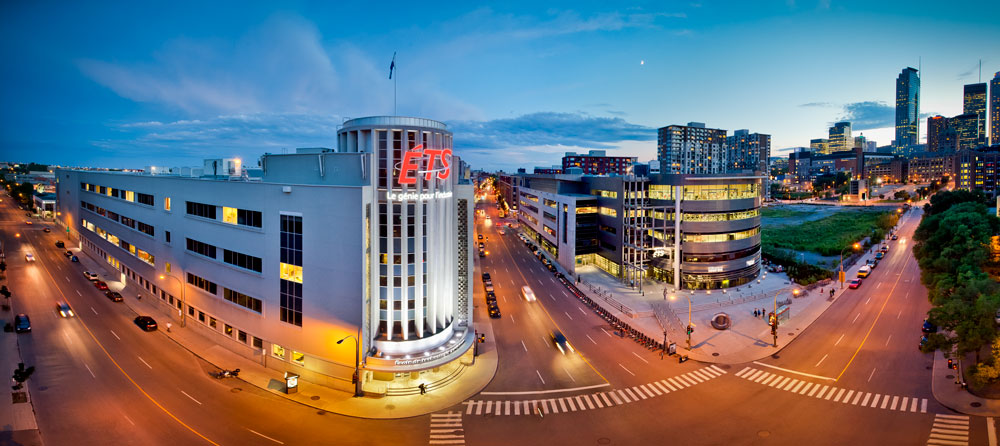
\includegraphics[width=0.75\textwidth]{Figures/vueEts.jpg} % Usage of the "width" parameter to constraint the with of the figure, respecting proportions. In this example, the width is set to 0.75 times the maximum text width (\textwidth), respecting the margins.
%	}
	% \\ \parbox{0.75\textwidth}{\caption{Test of a long caption, using a framebox and a %parbox to constrain the caption.}\label{fig:vueEts}} % Usage of a parbox to contrain the width of the caption, in this example fixed to the same width than the figure (0.75\textwidth). The decanat wants to avoid captions larger than the figure, if possible (i.e. if the figure is not too narrow, otherwise the caption would require too many lines)
%\end{figure}

%\lipsum[1] % Text filling, to have an example of the layout
Auditory processing is the ability of the central auditory nervous
system(CANS) to use and process auditory information
received peripherally by the two ears. Auditory processing
disorders (APD) are typically seen in individualswith normal
hearing sensitivity and are characterized by an inability of the
central auditory neurons to mediate higher-order auditory
processing skills (e.g., speech in noise, binaural processing,
temporal processing, and closure). Individuals with APD
manifest listening difficulties in challenging listening conditions,
show deficits in spatial location (localization) of
sounds, and face difficulties in decoding rapid rate stimuli \cite{American}.
The effects of APD can be devastating because as an input
disorder, it has the potential to impair the abilities for spoken
language comprehension, learning, and cognition in schoolage
children.
\par One of the main problems in identification of APD is that
this disorder often coexists with other comorbid conditions
in school-age children such as attention deficit disorders,
language learning disorders, and learning disabilities \cite{Jerger}.
This makes differential diagnosis of APD difficult. Also
audiologists routinely use primarily language-based auditory
processing measures for diagnosis of APD even though it
is not clear whether deficits on linguistic (verbal) tasks are
more likely to be associated with APD than nonlinguistic
(e.g., tonal) tasks. In a study by Rosen et al. \cite{Rosen}, it has
been shown that school-age children with suspected APD
exhibited poorer performance on auditory tests in both
verbal (Consonant Cluster Minimal Pairs) and tonal (Tallal
Discrimination Task) conditions, relative to age-matched
controls. There is also dispute regarding formulation of the
appropriate test battery for evaluation of APD (e.g., \cite{Cacacea}).
Cacace and Mc. Farland \cite{Cacaceb} argued that, for a diagnosis of
APD, testing should address the primary deficit in processing
of acoustic information in the auditory modality and deficits
should be shown to be absent or reduced in other (e.g., visual)
modalities. While this notion is disputed by other studies
\cite{Musiek, Moore}, there is consensus on the need for valid tools that
challenge listening in the auditory modality for school-age
children with APD.


The diagnosis encompasses a number of overlapping clinical syndromes (Jerger and Musiek, 2000; Hind, 2006), and its underlying pathological basis is poorly understood. Of those children complaining of symptoms consistent with APD, only around 5\% have an underlying structural or other obvious neurological cause (Chermak and Musiek, 1997).

\par On the other hand,  artificial intelligence (AI) is a self-running engine for growth in healthcare. According to Accenture analysis, when combined, key clinical health AI applications can potentially create \$150 billion in annual savings for the US healthcare economy by 2026. AI in health represents a collection of multiple technologies enabling machines to sense, comprehend, act and learn\footnote{ Accenture; “AI is the Future of Growth”} so they can perform administrative and clinical healthcare functions. Unlike legacy technologies that are only algorithms/ tools that complement a human, health AI today can truly augment human activity. With immense power to unleash improvements in cost, quality and access, AI is exploding in popularity. Growth in the AI health market is expected to reach \$6.6 billion by 2021--that’s a compound annual growth rate of 40\%. In just the next five years, the health AI market will grow more than 10x.\footnote{Frost \& Sullivan}. AI applications focus on Robot-assisted surgery, Virtual nursing assistance,  Administrative workflow assistance,  Fraud detection, Dosage error reduction, Connected machines, Clinical trail participant identifier, Preliminary diagnosis, Automated image diagnosis, and Cybersecurity\footnote{https://www.accenture.com}. 
\par Neural networks are adaptive statistical models based
on analogies with human brain structure that can learn to
estimate and iteratively change values of the parameters of
some population using specific input and output variables
\cite{Abdi}. An artificial neural network (ANN), often just called a
“neural network” (NN), is a mathematical model or computationalmodel
based on biological neural networks. Artificial
neural networks can be used to model complex relationships
between input and output variables and explain patterns
of data. The construction of the neural network typically
involves three different layers with feed-forward architecture.
This is the most popular network architecture in use today.
The input layer of this network is a set of input units, neurons
that are fully connected to the hidden layer with the hidden
units that are in turn fully connected to an output layer.
The output layer supplies the response of neural network
to the activation pattern applied to the input layer. Neural
network modeling has been used in healthcare research to
characterize and predict a wide variety of health-related
issues such as infant mortality \cite{Gismondi}, brain surgery decisions
\cite{Li}, pharmacokinetic parameters of antibiotics in severely ill
patients \cite{Yamamura}, and auditory dysfunction inAlzheimer’s disease
\cite{Krishnamurti}. Neural networks can be used to model cognitive processes
by a feed-forward, backward propagation algorithm
called multilayer perceptrons (MLPs). These networks usually
organize their units into several layers. The information
to be analyzed is fed to the first layer called the input layer,
followed by intermediate hidden layers, finally leading to
the output layer for processing \cite{Abdi}. Unlike multiple linear
regression models used to predict performance from known
variables, artificial neural networks need no prior knowledge
or assumptions because they can learn and generalize from
data that are even noisy or imperfect \cite{Keshavarzi}.
The current study was conducted to probe if reducing
extrinsic redundancy in the P300 Auditory Event-Related Potentials (P3AERP) task compromises auditory
processing in school-age children with and without APD.
Extrinsic redundancy can be reduced in several ways, but,
for the purposes of this study, two stimulus-related variables
(competing noise and rapid rates) were used. The rationale
for reducing the extrinsic redundancy was that competing
noise would limit spectral processing abilities needed to discriminate frequent and infrequent stimuli on the P3AERP
task while rapid presentation rates would stress the temporal
processing capabilities of the auditory system and these
would have particular influence on P3AERP latency and
amplitude measures in those children with reduced intrinsic
redundancy (children with APD). Neural network modeling
was performed statistically to discover hidden and nonlinear
associations between input (stimulus rate and competing
noise) and output variables (P3AERP latency and amplitude).

\end{introduction}

%%- Uncomment the literature review for a thesis by articles -%%
%\begin{literaturereview}

%\end{literaturereview}

%%- First demo chapter -%%
\chapter{Problem Definition.}


\section{Detect APD early}

There are a variety of possible behavioural indicators that a child may have APD. A diagnosis
can be made following testing by a specialized audiologist using specific tests. Some of
the skills evaluated by the audiologist will not develop in the child until age 8 or 9. Once diagnosed,
APD children often work with a speech therapist. APD is recognized as a learning
disability and should therefore be recognized as qualifying a child as an exceptional learner.
This means that once a diagnosis is made and recommendations are clearly stated in the audiologist’s
report, parents should request a school meeting to discuss how accommodations
and special education resources will be implemented. The children will be eligible for an FM
system (a headset the children wears to listen directly to the teacher/instructor via microphone)
to be placed in the classroom (see accommodations below). The cost of this system is an issue
when obtaining this device. A trial with the system is usually initiated to assess the benefits.
If several children in the classroom suffer from this disorder, a surround sound system can be
installed in the classroom. The signs and symptoms of APD is following:\footnote{http://kidshealth.org}
\begin{itemize}
	\item Difficulty hearing in noisy environments
	\item Frequently misunderstanding oral instructions/questions
	\item Says “huh” or “what” frequently
	\item Often needs directions or information repeated
	\item Difficulty remembering spoken information
	\item Difficulty with reading, comprehension, spelling, vocabulary, writing, or learning a foreign	language
\item Difficulty with phonics or distinguishing speech sounds
\item Difficulty with organizational skills
	\item Difficulty following multi-step directions
	\item Difficulty maintaining focus on an activity if other sounds are present or child is easily
	distracted by other sounds in the environment
	\item Difficulty following long conversations
	\item Difficulty taking notes
	\item Difficulty with verbal (word) math problems
	 
\end{itemize}

Switzerland). Each experimental series (i.e. hearing
test) was presented in alternating activation blocks and silent blocks of the same duration.
Following the stimuli in each activation block, individuals were asked to press a button (HPDT:
depending on whether the speech sounds were perceived as the same or different), or to repeat
softly the words they had heard (MST and DLT). Considering the normal familiarization test
results, vocal output was not recorded in detail in this setup. The probands were monitored
intermittently by listening to the audio output of the microphone built into the scanner. In this
field, there was no indication that response accuracy or reaction time were reduced or delayed,
respectively. fMRI scanning and data acquisition. Functional measurements were performed
on a 1.5 Tesla machine with a head coil (Magnetom Sonata, Siemens AG Medical Solutions,
Forchheim/Erlangen, Germany). The acquired EPI sequences covered the auditory cortex of
the temporal gyrus and the inferior portions of the frontal cortex. The total duration of each
MRI examination was approximately 30 minutes {\cite{-Friedrich}}.

\textbf{Therefore, our first problem is that how to identify, recognize, and diagnosing children
early with Auditory Processing Disorder (APD) based on their sentiment behavior, speech,
and response with the lowest cost.}
\section{Treading APD daily}
Auditory processing disorder is a neurological problem that cannot be treated by medication\footnote{https://www.additudemag.com}.
Hence, there are many non-medical ways to help your child with auditory processing disorder
succeed in the classroom and in life \footnote{https://www.understood.org} as following \footnote{https://www.asha.org}:
- Treating APD with Therapy: To overcome sound discrimination problem (e.g., the professional
will train your child’s brain to differentiate sounds, To sharpen auditory memory
(e.g., an audiologist will use sequencing routines), and To manage language-processing
problems (e.g., the therapist will train and encourage your child to ask a teacher, adult, or
peer to repeat or rephrase an instruction or comment, etc.,)
- Treating APD with Lifestyle Changes: At school (e.g., Improve classroom acoustics, Seat
children near the front of the class, Provide attention prompts, Streamline communication,
Use visual aids, Build in breaks, Use a microphone and headset, and deep communication
with the children) on the other hand, at home (e.g., Boost auditory attention with games and
tapes, Provide a structure to help your child focus in chaotic environments, Speak concisely,
etc.,)
We observe that the best way to treat the APD is making the information more clearly and
concisely in parallel with monitoring the progress of treatment. \textbf{So our second problem is
that how to help users to solve their issues above, comment the training therapy to them,
and monitor the progress with the low cost and convenience.}

\chapter{Challenges and Object}

\section{Challenges}
\begin{itemize}
	\item  Unlike people, machines have been notoriously unreliable at recognizing speech in the
	presence of noise, especially when the noise is background speech. Speech recognition
	technology is becoming increasingly ubiquitous and is now being used for dictating text
	and commands to computers, phones and GPS devices. Hence, the first challenges is speech
	recognition from multiple speakers.
	\item  The challenge comes from the discrete nature of text samples. The resulting non differentiability
	hinders the use of global discriminators that assess generated samples and back-propagate
	gradients to guide the optimization of generators in a holistic manner, as shown to be highly
	effective in continuous image generation and representation modeling \cite{C. Xi, Lindbo,Diederik}. A number
	of recent approaches attempt to address the non-differentiability through policy learning
	\cite{Alexey} which tends to suffer from high variance during training, or continuous approximations
	\cite{Lantao,Yizhe} where only preliminary qualitative results are presented. As an alternative to the
	discriminator based learning, semi-supervised \cite{Diederik} minimize element-wise reconstruction
	error on observed examples and are applicable to discrete visibles. This, however, loses the
	holistic view of full sentences and can be inferior especially for modeling global abstract attributes
	(e.g., sentiment). Another challenge for controllable generation relates to learning
	disentangled latent representations. Interpretability expects each part of the latent representation
	to govern and only focus on one aspect of the samples. Prior methods \cite{C. Xi,Augustus}
	on structured toward controlled generation of text dependence property on the full latent
	representation, and varying individual code may result in unexpected variation of other unspecified
	attributes besides the desired one. Therefore, the second challenges is understand
	the semantic, generating and evaluate different level of complexity sentences in the many
	context to multiple simpler sentences
\end{itemize}

\section{Objectives}
Propose an AI model (virtual assitant) to assist in diagnosing, monitoring, and training of the
children with Auditory Processing Disorder (APD)
\begin{itemize}
	\item Diagnose APD symptoms based on conversation with the candidate children
	\item Create a training therapy model assistance (adaptable)
	\item Make a method to monitor the progress of APD treatment
	
\end{itemize}

%%- Second demo chapter -%%
\chapter{RESEARCH METHODOLOGY}

\section{Diagnose APD symptoms based on conversation with the candidate children}

The datasets in real life are much more complex. We first have to understand it, collect it from
various sources and arrange it in a format which is ready for processing. This is even more
difficult when the data is in an unstructured format such as video or audio. This is so because
you would have to represent video/audio data in a standard way for it to be useful for analysis
\subsection {Sound analysis}
By considering the conversation between the APD candidate children with the computer as the
methods for processing audio with deep neural networks are improving, we can only begin
to imagine the difficult problems we could solve ere are a few of my imaginations for deep
learning in real time audio processing and sound analysis:
\begin{itemize}
	\item  Noise canceling, removing only certain elements like car traffic
	\item  Selective terms frequency, couting certain elements like "huh", "what" or some stutter
	words.
	\item  Speech processing, changing speaker, dialect or language in recordings
	\item  Frequently misunderstanding oral instructions/questions
	\item  Often needs directions or information repeated
\end{itemize}

Our speech capability analyzes not what is said, but how it is said, observing changes in speech
paralinguistics, tone, loudness, tempo, and voice quality to distinguish speech events, emotions,
and gender. The underlying low latency approach is key to enabling the development of
real-time emotion-aware apps and devices.





\subsection{Facial sentiment behavior analysis}
The face is an observable proxy for a wide range of factors, like your life history, your development
factors, whether you’re healthy. Faces contain a significant amount of information,
and using large datasets of photos, sophisticated computer programs can uncover trends and
learn how to distinguish key traits with a high rate of accuracy \footnote{https://www.theguardian.com}. Our Emotion AI unobtrusively
measures unfiltered and unbiased facial expressions of emotion, using any optical sensor
or just a standard webcam. Our technology first identifies a human face in real time or in an
image or video. Computer vision algorithms identify key landmarks on the face – for example,
the corners of your eyebrows, the tip of your nose, the corners of your mouth. Deep learning
algorithms then analyze pixels in those regions to classify facial expressions. Combinations of
these facial expressions are then mapped to emotions. In our products, we measure 7 emotion
metrics: anger, contempt, disgust, fear, joy, sadness and surprise. Hence by anaylsis the facial
sentiment behavior we can detect some APD symptoms:
\begin{itemize}
	\item  Difficulty with reading, comprehension, spelling, vocabulary, writing, or learning a foreign
	language
		\item  Difficulty with phonics or distinguishing speech sounds
		\item  Difficulty with organizational skills
		\item  Difficulty maintaining focus on an activity if other sounds are present or child is easily
	distracted by other sounds in the environment
		\item  Difficulty following long conversations
		\item  Difficulty taking notes
	
\end{itemize}

\section{A training adaptable therapy model assitance}
In this work we study transferring the idea of collaborative filtering to the domain of clinical
decision support systems by developing a recommender system aiming at predicting the adequacy
of various therapies for a given patient at a given time. Therefore, two methodologies for
therapy adequacy estimation, a Collaborative Recommender and a hybrid Demographicbased
Recommender, are compared. A physician can incorporate that information into his decision
on the therapy to be chosen. The exemplary recommender system is developed targeting therapy
recommendations for patients suffering from the auditory processing disorder

\section{ A monitoring the progress of APD treatment}
APD patient monitoring is one of the important application of MedicBot. This allows a faster
and cost- efficient way of conducting regular doctor-to-patient consults to assess the patient’s
current state and clinical results at a distance. This has been developed to resemble human to
machine consultation through video conferencing and the connection of digital medical devices
to take and record the patient’s clinical data (e.g., symptoms, tranining therapy exam and its’
plan, the automatic diagnosing APD). The objective of this trend is to provide accessibility,
ease, efficiency, and reduce costs compared to physical patient monitoring.

%%%%%%%%%%%%%%%%%%%%%%%%%%%%%%%%%%%%%%%%%%%%%%%%%%%
% BIBLIOGRAPHY AND REFERENCES
%%%%%%%%%%%%%%%%%%%%%%%%%%%%%%%%%%%%%%%%%%%%%%%%%%%

\begin{thebibliography}{9}

	\bibitem{American} American-Speech-Language-Hearing Association (ASHA), (Central) Auditory Processing
	Disorders—The Role of the Audiologist. [Position Statement], American-Speech-
	Language- Hearing Association, 2005, http://www.asha.org/policy.
	\bibitem{Jerger} J. Jerger and F.Musiek, “Report of the consensus conference on the diagnosis of auditory
	processing disorders in school-aged children,” Journal of the American Academy of Audiology,
	vol. 11, no. 9, pp. 467–474, 2000.
\bibitem{Rosen} S. Rosen, M. Cohen, and I. Vanniasegaram, “Auditory and cognitive abilities of children suspected of auditory processing disorder (APD),” International Journal of Pediatric
	Otorhinolaryngology, vol. 74, no. 6, pp. 594–600, 2010.
	\bibitem{Cacacea} A. T. Cacace and D. J.McFarland, “The importance of modality specificity in diagnosing
	central auditory processing disorder,” Journal of the American Academy of Audiology,
	vol. 14, no. 2, pp. 112–113, 2005.
	\bibitem{Cacaceb} A. T. Cacace and D. J. McFarland, “Factors influencing tests of auditory processing: a
	perspective on current issues and relevant concerns,” Journal of the American Academy of
	Audiology, vol. 24, no. 7, pp. 572–589, 2013.
	\bibitem{Musiek} F. E. Musiek, T. J. Bellis, and G. D. Chermak, “Nonmodularity of the central auditory
	nervous system: implication for (central) auditory processing disorder,” Journal of the
	American Academy of Audiology, vol. 14, no. 2, pp. 128–138, 2005.
\bibitem{Moore} D. R. Moore and M. A. Ferguson, “It is neither necessary nor desirable to test for abnormalities
	in other modalities when diagnosing auditory processing disorder (APD),” Journal
	of the American Academy of Audiology, vol. 25, no. 7, pp. 695–696, 2014.
\bibitem{Abdi} H. Abdi, “Neural networks,” in Encyclopedia of Social Sciences Research Methods,
	Sage,Thousand Oaks, Calif, USA, 2003.
	16
\bibitem{Gismondi} R. C. Gismondi, R. M. V. R. Almeida, and A. F. C. Infantosi, “Artificial neural networks
	for infant mortality modelling,” Computer Methods and Programs in Biomedicine, vol. 69,
	no. 3, pp. 237–247, 2002.
\bibitem{Li} Y.-C. Li, L. Liu, W.-T. Chiu, and W.-S. Jian, “Neural network modeling for surgical
	decisions on traumatic brain injury patients,” International Journal of Medical Informatics,
	vol. 57, no. 1, pp. 1–9, 2000.
\bibitem{Yamamura} S. Yamamura, “Clinical application of artificial neural network (ANN) modeling to predict
	pharmacokinetic parameters of severely ill patients,” Advanced Drug Delivery Reviews,
	vol. 55, no. 9, pp. 1233–1251, 2003.
\bibitem{Krishnamurti} S. Krishnamurti, L. Drake, and J. King, “Neural network modeling of central auditory
	dysfunction in Alzheimer’s disease,” Neural Networks, vol. 24, no. 6, pp. 646–651, 2011.
\bibitem{Keshavarzi} A. Keshavarzi and F. Sarmadian, “Comparison of artificial neural network and multivariate
	regression methods in prediction of soil cation exchange capacity,” International
	Journal of Environmental and Earth Sciences, vol. 15, no. 2, pp. 167–174, 2010.
\bibitem{-Friedrich} S. B.-Friedrich, Y. Broecker, M. Knoergen, and S. Koesling, "Development of fMRI Tests
	for Children with Central Auditory Processing Disorders", in ViVo 24: 201-210 (2010)
\bibitem{C. Xi} C. Xi, D. Yan, H. Rein, S. John, S. Ilya, and A. Pieter, "InfoGAN: Interpretable representation
	learning by information maximizing generative adversarial nets", in Advances in
	Neural Information Processing Systems, pp. 2172–2180, 2016.
\bibitem{Lindbo} L. A. B. Lindbo, S. S. Kaae, and W. Ole, "Autoencoding beyond pixels using a learned
	similarity metric", in ICML, 2016.
\bibitem{Alexey} D. Alexey and B. Thomas, "Generating images with perceptual similarity metrics based
	on deep networks", in arXiv preprint arXiv:1602.02644, 2016.
\bibitem{Lantao} Y. Lantao, Z. Weinan, W. Jun, and Y. Yong, "SeqGAN: sequence generative adversarial
	nets with policy gradient", in AAAI, 2017

\bibitem{Yizhe} Z. Yizhe, G. Zhe, and C. Lawrence, "Generating text via adversarial training", in NIPS
	Workshop on Adversarial Training, 2016
\bibitem{Matt} K. Matt and H.-. Jos, "GANs for sequences of discrete elements with the Gumbel-softmax
	distribution", in arXiv preprint arXiv:1611.04051, 2016
\bibitem{Diederik} K. Diederik, P. Mohamed, S. Rezende, D. Jimenez, andW. Max, "Semi-supervised learning
	with deep generative models", in Advances in Neural Information Processing Systems,
	pp. 3581–3589, 2014.

\bibitem{Augustus} O. Augustus, O. Christopher, and . Jonathon"Conditional image synthesis with auxiliary
	classifier GANs", in arXiv preprint arXiv:1610.09585, 2016.
	\end{thebibliography}

\end{document}
